\documentclass[1p]{elsarticle_modified}
%\bibliographystyle{elsarticle-num}

%\usepackage[colorlinks]{hyperref}
%\usepackage{abbrmath_seonhwa} %\Abb, \Ascr, \Acal ,\Abf, \Afrak
\usepackage{amsfonts}
\usepackage{amssymb}
\usepackage{amsmath}
\usepackage{amsthm}
\usepackage{scalefnt}
\usepackage{amsbsy}
\usepackage{kotex}
\usepackage{caption}
\usepackage{subfig}
\usepackage{color}
\usepackage{graphicx}
\usepackage{xcolor} %% white, black, red, green, blue, cyan, magenta, yellow
\usepackage{float}
\usepackage{setspace}
\usepackage{hyperref}

\usepackage{tikz}
\usetikzlibrary{arrows}

\usepackage{multirow}
\usepackage{array} % fixed length table
\usepackage{hhline}

%%%%%%%%%%%%%%%%%%%%%
\makeatletter
\renewcommand*\env@matrix[1][\arraystretch]{%
	\edef\arraystretch{#1}%
	\hskip -\arraycolsep
	\let\@ifnextchar\new@ifnextchar
	\array{*\c@MaxMatrixCols c}}
\makeatother %https://tex.stackexchange.com/questions/14071/how-can-i-increase-the-line-spacing-in-a-matrix
%%%%%%%%%%%%%%%

\usepackage[normalem]{ulem}

\newcommand{\msout}[1]{\ifmmode\text{\sout{\ensuremath{#1}}}\else\sout{#1}\fi}
%SOURCE: \msout is \stkout macro in https://tex.stackexchange.com/questions/20609/strikeout-in-math-mode

\newcommand{\cancel}[1]{
	\ifmmode
	{\color{red}\msout{#1}}
	\else
	{\color{red}\sout{#1}}
	\fi
}

\newcommand{\add}[1]{
	{\color{blue}\uwave{#1}}
}

\newcommand{\replace}[2]{
	\ifmmode
	{\color{red}\msout{#1}}{\color{blue}\uwave{#2}}
	\else
	{\color{red}\sout{#1}}{\color{blue}\uwave{#2}}
	\fi
}

\newcommand{\Sol}{\mathcal{S}} %segment
\newcommand{\D}{D} %diagram
\newcommand{\A}{\mathcal{A}} %arc


%%%%%%%%%%%%%%%%%%%%%%%%%%%%%5 test

\def\sl{\operatorname{\textup{SL}}(2,\Cbb)}
\def\psl{\operatorname{\textup{PSL}}(2,\Cbb)}
\def\quan{\mkern 1mu \triangleright \mkern 1mu}

\theoremstyle{definition}
\newtheorem{thm}{Theorem}[section]
\newtheorem{prop}[thm]{Proposition}
\newtheorem{lem}[thm]{Lemma}
\newtheorem{ques}[thm]{Question}
\newtheorem{cor}[thm]{Corollary}
\newtheorem{defn}[thm]{Definition}
\newtheorem{exam}[thm]{Example}
\newtheorem{rmk}[thm]{Remark}
\newtheorem{alg}[thm]{Algorithm}

\newcommand{\I}{\sqrt{-1}}
\begin{document}

%\begin{frontmatter}
%
%\title{Boundary parabolic representations of knots up to 8 crossings}
%
%%% Group authors per affiliation:
%\author{Yunhi Cho} 
%\address{Department of Mathematics, University of Seoul, Seoul, Korea}
%\ead{yhcho@uos.ac.kr}
%
%
%\author{Seonhwa Kim} %\fnref{s_kim}}
%\address{Center for Geometry and Physics, Institute for Basic Science, Pohang, 37673, Korea}
%\ead{ryeona17@ibs.re.kr}
%
%\author{Hyuk Kim}
%\address{Department of Mathematical Sciences, Seoul National University, Seoul 08826, Korea}
%\ead{hyukkim@snu.ac.kr}
%
%\author{Seokbeom Yoon}
%\address{Department of Mathematical Sciences, Seoul National University, Seoul, 08826,  Korea}
%\ead{sbyoon15@snu.ac.kr}
%
%\begin{abstract}
%We find all boundary parabolic representation of knots up to 8 crossings.
%
%\end{abstract}
%\begin{keyword}
%    \MSC[2010] 57M25 
%\end{keyword}
%
%\end{frontmatter}

%\linenumbers
%\tableofcontents
%
\newcommand\colored[1]{\textcolor{white}{\rule[-0.35ex]{0.8em}{1.4ex}}\kern-0.8em\color{red} #1}%
%\newcommand\colored[1]{\textcolor{white}{ #1}\kern-2.17ex	\textcolor{white}{ #1}\kern-1.81ex	\textcolor{white}{ #1}\kern-2.15ex\color{red}#1	}

{\Large $\underline{12a_{0579}~(K12a_{0579})}$}

\setlength{\tabcolsep}{10pt}
\renewcommand{\arraystretch}{1.6}
\vspace{1cm}\begin{tabular}{m{100pt}>{\centering\arraybackslash}m{274pt}}
\multirow{5}{120pt}{
	\centering
	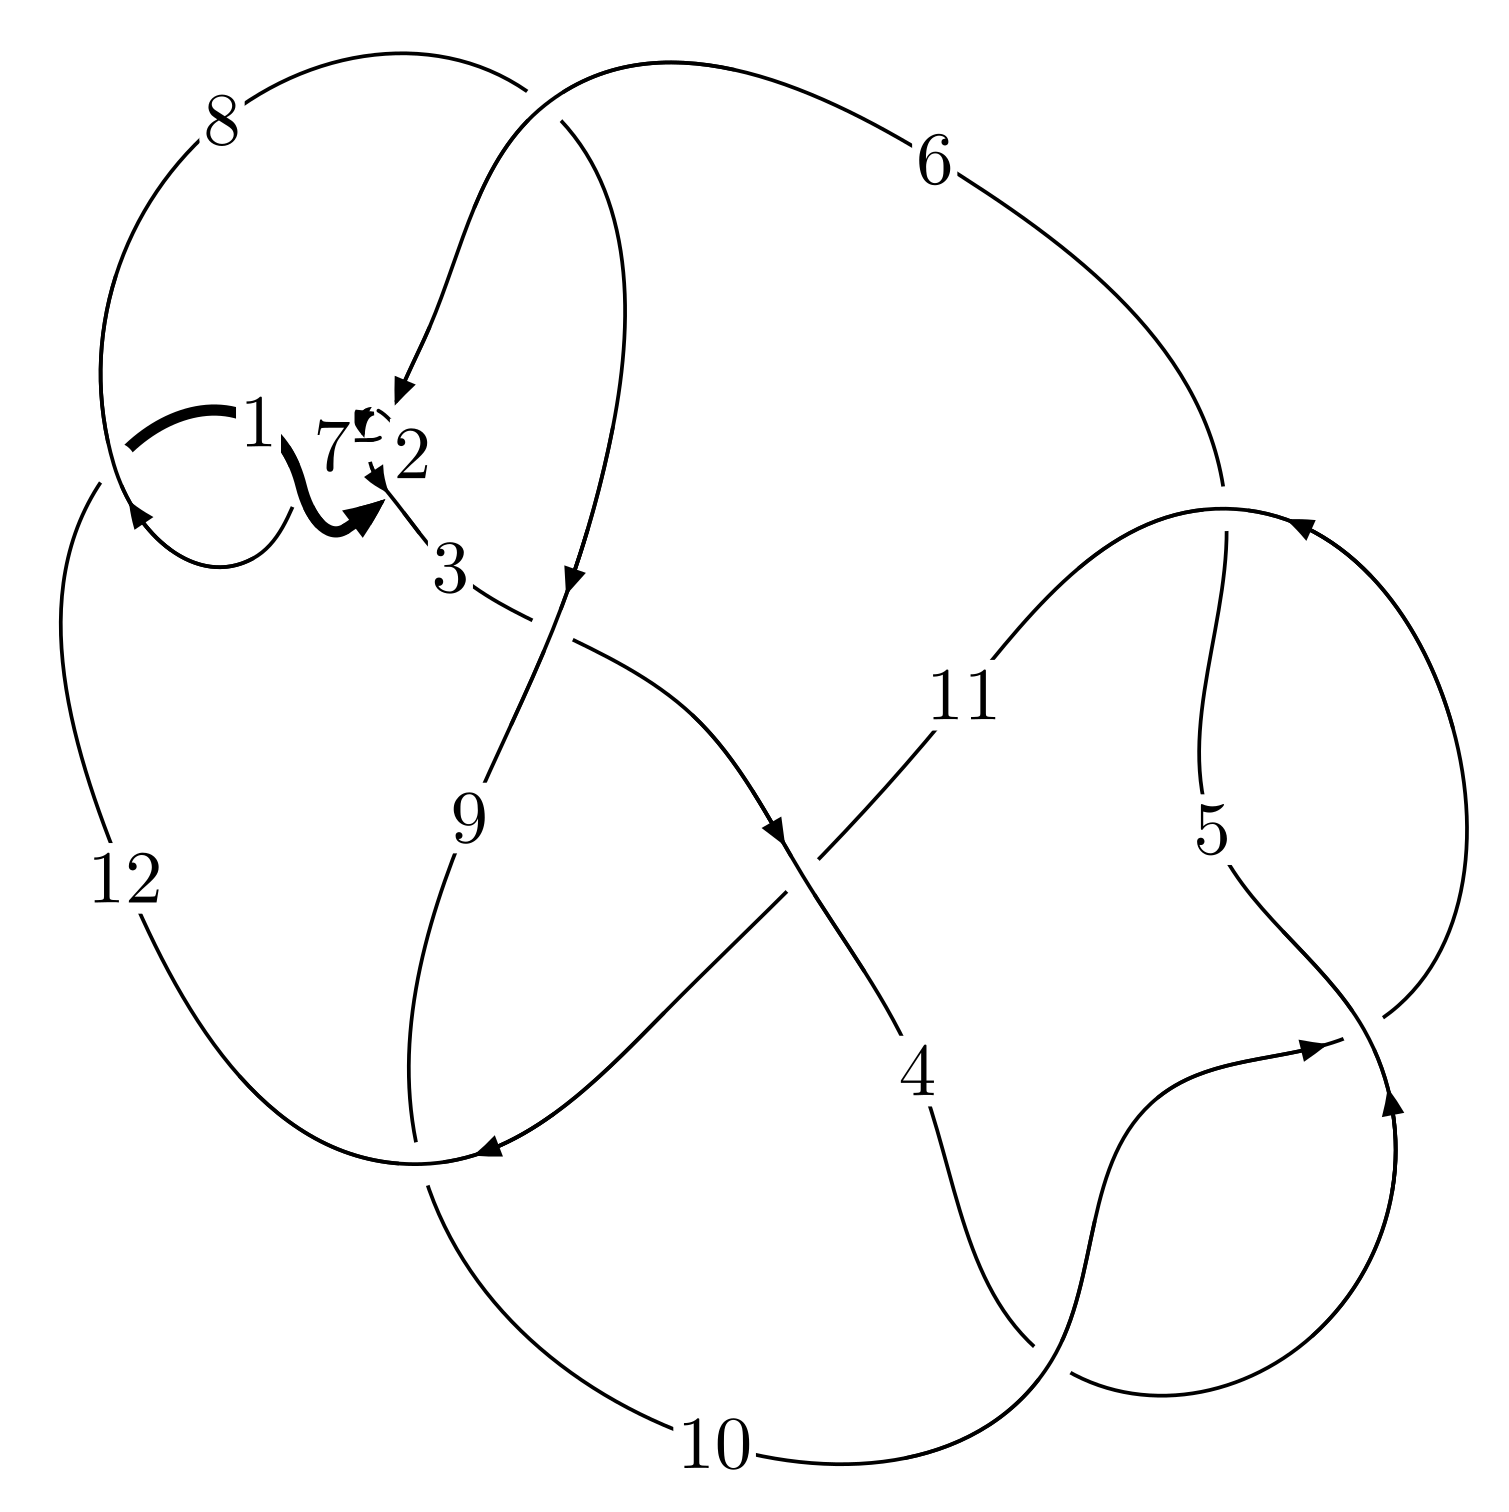
\includegraphics[width=112pt]{../../../GIT/diagram.site/Diagrams/png/1380_12a_0579.png}\\
\ \ \ A knot diagram\footnotemark}&
\allowdisplaybreaks
\textbf{Linearized knot diagam} \\
\cline{2-2}
 &
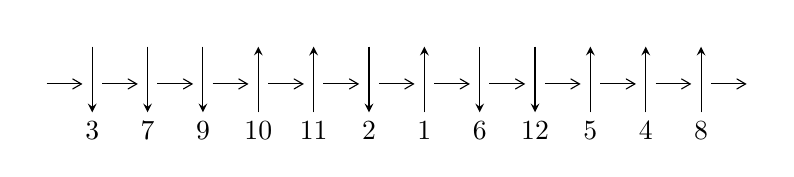
\begin{tikzpicture}[x=20pt, y=17pt]
	% nodes
	\node (C0) at (0, 0) {};
	\node (C1) at (1, 0) {};
	\node (C1U) at (1, +1) {};
	\node (C1D) at (1, -1) {3};

	\node (C2) at (2, 0) {};
	\node (C2U) at (2, +1) {};
	\node (C2D) at (2, -1) {7};

	\node (C3) at (3, 0) {};
	\node (C3U) at (3, +1) {};
	\node (C3D) at (3, -1) {9};

	\node (C4) at (4, 0) {};
	\node (C4U) at (4, +1) {};
	\node (C4D) at (4, -1) {10};

	\node (C5) at (5, 0) {};
	\node (C5U) at (5, +1) {};
	\node (C5D) at (5, -1) {11};

	\node (C6) at (6, 0) {};
	\node (C6U) at (6, +1) {};
	\node (C6D) at (6, -1) {2};

	\node (C7) at (7, 0) {};
	\node (C7U) at (7, +1) {};
	\node (C7D) at (7, -1) {1};

	\node (C8) at (8, 0) {};
	\node (C8U) at (8, +1) {};
	\node (C8D) at (8, -1) {6};

	\node (C9) at (9, 0) {};
	\node (C9U) at (9, +1) {};
	\node (C9D) at (9, -1) {12};

	\node (C10) at (10, 0) {};
	\node (C10U) at (10, +1) {};
	\node (C10D) at (10, -1) {5};

	\node (C11) at (11, 0) {};
	\node (C11U) at (11, +1) {};
	\node (C11D) at (11, -1) {4};

	\node (C12) at (12, 0) {};
	\node (C12U) at (12, +1) {};
	\node (C12D) at (12, -1) {8};
	\node (C13) at (13, 0) {};

	% arrows
	\draw[->,>={angle 60}]
	(C0) edge (C1) (C1) edge (C2) (C2) edge (C3) (C3) edge (C4) (C4) edge (C5) (C5) edge (C6) (C6) edge (C7) (C7) edge (C8) (C8) edge (C9) (C9) edge (C10) (C10) edge (C11) (C11) edge (C12) (C12) edge (C13) ;	\draw[->,>=stealth]
	(C1U) edge (C1D) (C2U) edge (C2D) (C3U) edge (C3D) (C4D) edge (C4U) (C5D) edge (C5U) (C6U) edge (C6D) (C7D) edge (C7U) (C8U) edge (C8D) (C9U) edge (C9D) (C10D) edge (C10U) (C11D) edge (C11U) (C12D) edge (C12U) ;
	\end{tikzpicture} \\
\hhline{~~} \\& 
\textbf{Solving Sequence} \\ \cline{2-2} 
 &
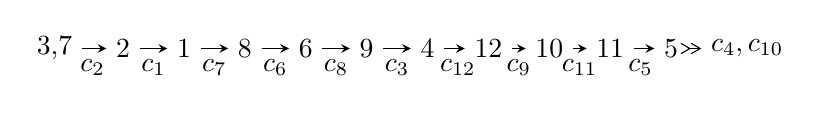
\begin{tikzpicture}[x=22pt, y=7pt]
	% node
	\node (A0) at (-1/8, 0) {3,7};
	\node (A1) at (1, 0) {2};
	\node (A2) at (2, 0) {1};
	\node (A3) at (3, 0) {8};
	\node (A4) at (4, 0) {6};
	\node (A5) at (5, 0) {9};
	\node (A6) at (6, 0) {4};
	\node (A7) at (7, 0) {12};
	\node (A8) at (8, 0) {10};
	\node (A9) at (9, 0) {11};
	\node (A10) at (10, 0) {5};
	\node (C1) at (1/2, -1) {$c_{2}$};
	\node (C2) at (3/2, -1) {$c_{1}$};
	\node (C3) at (5/2, -1) {$c_{7}$};
	\node (C4) at (7/2, -1) {$c_{6}$};
	\node (C5) at (9/2, -1) {$c_{8}$};
	\node (C6) at (11/2, -1) {$c_{3}$};
	\node (C7) at (13/2, -1) {$c_{12}$};
	\node (C8) at (15/2, -1) {$c_{9}$};
	\node (C9) at (17/2, -1) {$c_{11}$};
	\node (C10) at (19/2, -1) {$c_{5}$};
	\node (A11) at (45/4, 0) {$c_{4},c_{10}$};

	% edge
	\draw[->,>=stealth]	
	(A0) edge (A1) (A1) edge (A2) (A2) edge (A3) (A3) edge (A4) (A4) edge (A5) (A5) edge (A6) (A6) edge (A7) (A7) edge (A8) (A8) edge (A9) (A9) edge (A10) ;
	\draw[->>,>={angle 60}]	
	(A10) edge (A11);
\end{tikzpicture} \\ 

\end{tabular} \\

\footnotetext{
The image of knot diagram is generated by the software ``\textbf{Draw programme}" developed by Andrew Bartholomew(\url{http://www.layer8.co.uk/maths/draw/index.htm\#Running-draw}), where we modified some parts for our purpose(\url{https://github.com/CATsTAILs/LinksPainter}).
}\phantom \\ \newline 
\centering \textbf{Ideals for irreducible components\footnotemark of $X_{\text{par}}$} 
 
\begin{align*}
I^u_{1}&=\langle 
u^{87}+2 u^{86}+\cdots-3 u-1\rangle \\
I^u_{2}&=\langle 
u-1\rangle \\
\\
\end{align*}
\raggedright * 2 irreducible components of $\dim_{\mathbb{C}}=0$, with total 88 representations.\\
\footnotetext{All coefficients of polynomials are rational numbers. But the coefficients are sometimes approximated in decimal forms when there is not enough margin.}
\newpage
\renewcommand{\arraystretch}{1}
\centering \section*{I. $I^u_{1}= \langle u^{87}+2 u^{86}+\cdots-3 u-1 \rangle$}
\flushleft \textbf{(i) Arc colorings}\\
\begin{tabular}{m{7pt} m{180pt} m{7pt} m{180pt} }
\flushright $a_{3}=$&$\begin{pmatrix}1\\0\end{pmatrix}$ \\
\flushright $a_{7}=$&$\begin{pmatrix}0\\u\end{pmatrix}$ \\
\flushright $a_{2}=$&$\begin{pmatrix}1\\- u^2\end{pmatrix}$ \\
\flushright $a_{1}=$&$\begin{pmatrix}- u^2+1\\- u^2\end{pmatrix}$ \\
\flushright $a_{8}=$&$\begin{pmatrix}u^5-2 u^3+u\\u^5- u^3+u\end{pmatrix}$ \\
\flushright $a_{6}=$&$\begin{pmatrix}u\\- u^3+u\end{pmatrix}$ \\
\flushright $a_{9}=$&$\begin{pmatrix}- u^9+2 u^7- u^5-2 u^3+u\\u^{11}-3 u^9+4 u^7- u^5- u^3+u\end{pmatrix}$ \\
\flushright $a_{4}=$&$\begin{pmatrix}- u^{20}+5 u^{18}-11 u^{16}+10 u^{14}+2 u^{12}-13 u^{10}+9 u^8-3 u^4+u^2+1\\u^{22}-6 u^{20}+17 u^{18}-26 u^{16}+20 u^{14}-13 u^{10}+10 u^8- u^6-2 u^4+u^2\end{pmatrix}$ \\
\flushright $a_{12}=$&$\begin{pmatrix}- u^8+3 u^6-3 u^4+1\\- u^8+2 u^6-2 u^4\end{pmatrix}$ \\
\flushright $a_{10}=$&$\begin{pmatrix}- u^{27}+8 u^{25}+\cdots+4 u^5- u^3\\- u^{27}+7 u^{25}+\cdots- u^3+u\end{pmatrix}$ \\
\flushright $a_{11}=$&$\begin{pmatrix}u^{50}-13 u^{48}+\cdots+u^2+1\\- u^{52}+14 u^{50}+\cdots-6 u^8- u^4\end{pmatrix}$ \\
\flushright $a_{5}=$&$\begin{pmatrix}u^{76}-21 u^{74}+\cdots+u^2+1\\u^{76}-20 u^{74}+\cdots+10 u^8- u^4\end{pmatrix}$\\&\end{tabular}
\flushleft \textbf{(ii) Obstruction class $= -1$}\\~\\
\flushleft \textbf{(iii) Cusp Shapes $= 4 u^{86}-92 u^{84}+\cdots-4 u^2+6$}\\~\\
\newpage\renewcommand{\arraystretch}{1}
\flushleft \textbf{(iv) u-Polynomials at the component}\newline \\
\begin{tabular}{m{50pt}|m{274pt}}
Crossings & \hspace{64pt}u-Polynomials at each crossing \\
\hline $$\begin{aligned}c_{1}\end{aligned}$$&$\begin{aligned}
&u^{87}+46 u^{86}+\cdots- u+1
\end{aligned}$\\
\hline $$\begin{aligned}c_{2},c_{6}\end{aligned}$$&$\begin{aligned}
&u^{87}-2 u^{86}+\cdots-3 u+1
\end{aligned}$\\
\hline $$\begin{aligned}c_{3}\end{aligned}$$&$\begin{aligned}
&u^{87}-2 u^{86}+\cdots-15553 u+1789
\end{aligned}$\\
\hline $$\begin{aligned}c_{4},c_{5},c_{10}\end{aligned}$$&$\begin{aligned}
&u^{87}-39 u^{85}+\cdots- u+1
\end{aligned}$\\
\hline $$\begin{aligned}c_{7},c_{12}\end{aligned}$$&$\begin{aligned}
&u^{87}-3 u^{86}+\cdots+59 u+11
\end{aligned}$\\
\hline $$\begin{aligned}c_{8}\end{aligned}$$&$\begin{aligned}
&u^{87}-12 u^{86}+\cdots+3 u+1
\end{aligned}$\\
\hline $$\begin{aligned}c_{9}\end{aligned}$$&$\begin{aligned}
&u^{87}-18 u^{86}+\cdots+65191 u-4073
\end{aligned}$\\
\hline $$\begin{aligned}c_{11}\end{aligned}$$&$\begin{aligned}
&u^{87}-3 u^{86}+\cdots-3 u+11
\end{aligned}$\\
\hline
\end{tabular}\\~\\
\newpage\renewcommand{\arraystretch}{1}
\flushleft \textbf{(v) Riley Polynomials at the component}\newline \\
\begin{tabular}{m{50pt}|m{274pt}}
Crossings & \hspace{64pt}Riley Polynomials at each crossing \\
\hline $$\begin{aligned}c_{1}\end{aligned}$$&$\begin{aligned}
&y^{87}-10 y^{86}+\cdots+3 y-1
\end{aligned}$\\
\hline $$\begin{aligned}c_{2},c_{6}\end{aligned}$$&$\begin{aligned}
&y^{87}-46 y^{86}+\cdots- y-1
\end{aligned}$\\
\hline $$\begin{aligned}c_{3}\end{aligned}$$&$\begin{aligned}
&y^{87}-22 y^{86}+\cdots+148162943 y-3200521
\end{aligned}$\\
\hline $$\begin{aligned}c_{4},c_{5},c_{10}\end{aligned}$$&$\begin{aligned}
&y^{87}-78 y^{86}+\cdots- y-1
\end{aligned}$\\
\hline $$\begin{aligned}c_{7},c_{12}\end{aligned}$$&$\begin{aligned}
&y^{87}+69 y^{86}+\cdots-1579 y-121
\end{aligned}$\\
\hline $$\begin{aligned}c_{8}\end{aligned}$$&$\begin{aligned}
&y^{87}+2 y^{86}+\cdots+187 y-1
\end{aligned}$\\
\hline $$\begin{aligned}c_{9}\end{aligned}$$&$\begin{aligned}
&y^{87}+26 y^{86}+\cdots-406378973 y-16589329
\end{aligned}$\\
\hline $$\begin{aligned}c_{11}\end{aligned}$$&$\begin{aligned}
&y^{87}-3 y^{86}+\cdots+581 y-121
\end{aligned}$\\
\hline
\end{tabular}\\~\\
\newpage\flushleft \textbf{(vi) Complex Volumes and Cusp Shapes}
$$\begin{array}{c|c|c}  
\text{Solutions to }I^u_{1}& \I (\text{vol} + \sqrt{-1}CS) & \text{Cusp shape}\\
 \hline 
\begin{aligned}
u &= -0.966141 + 0.257989 I\end{aligned}
 & \phantom{-}3.05247 - 1.13677 I & \phantom{-0.000000 } 0 \\ \hline\begin{aligned}
u &= -0.966141 - 0.257989 I\end{aligned}
 & \phantom{-}3.05247 + 1.13677 I & \phantom{-0.000000 } 0 \\ \hline\begin{aligned}
u &= -0.884260 + 0.473666 I\end{aligned}
 & \phantom{-}1.43118 + 4.23576 I & \phantom{-0.000000 } 0 \\ \hline\begin{aligned}
u &= -0.884260 - 0.473666 I\end{aligned}
 & \phantom{-}1.43118 - 4.23576 I & \phantom{-0.000000 } 0 \\ \hline\begin{aligned}
u &= -0.840538 + 0.517807 I\end{aligned}
 & \phantom{-}1.69738 + 3.45223 I & \phantom{-0.000000 } 0 \\ \hline\begin{aligned}
u &= -0.840538 - 0.517807 I\end{aligned}
 & \phantom{-}1.69738 - 3.45223 I & \phantom{-0.000000 } 0 \\ \hline\begin{aligned}
u &= \phantom{-}0.862004 + 0.537117 I\end{aligned}
 & \phantom{-}0.53831 - 7.10255 I & \phantom{-0.000000 } 0 \\ \hline\begin{aligned}
u &= \phantom{-}0.862004 - 0.537117 I\end{aligned}
 & \phantom{-}0.53831 + 7.10255 I & \phantom{-0.000000 } 0 \\ \hline\begin{aligned}
u &= \phantom{-}0.818200 + 0.544961 I\end{aligned}
 & \phantom{-}7.81764 - 1.63453 I & \phantom{-}7.64996 + 3.75286 I \\ \hline\begin{aligned}
u &= \phantom{-}0.818200 - 0.544961 I\end{aligned}
 & \phantom{-}7.81764 + 1.63453 I & \phantom{-}7.64996 - 3.75286 I \\ \hline\begin{aligned}
u &= -1.014630 + 0.076379 I\end{aligned}
 & -3.56476 + 3.14041 I & \phantom{-0.000000 } 0 \\ \hline\begin{aligned}
u &= -1.014630 - 0.076379 I\end{aligned}
 & -3.56476 - 3.14041 I & \phantom{-0.000000 } 0 \\ \hline\begin{aligned}
u &= -0.862976 + 0.550546 I\end{aligned}
 & \phantom{-}6.01709 + 10.55840 I & \phantom{-0.000000 } 0 \\ \hline\begin{aligned}
u &= -0.862976 - 0.550546 I\end{aligned}
 & \phantom{-}6.01709 - 10.55840 I & \phantom{-0.000000 } 0 \\ \hline\begin{aligned}
u &= \phantom{-}1.034630 + 0.100691 I\end{aligned}
 & \phantom{-}1.61270 - 6.52842 I & \phantom{-0.000000 } 0 \\ \hline\begin{aligned}
u &= \phantom{-}1.034630 - 0.100691 I\end{aligned}
 & \phantom{-}1.61270 + 6.52842 I & \phantom{-0.000000 } 0 \\ \hline\begin{aligned}
u &= \phantom{-}0.877745 + 0.381441 I\end{aligned}
 & -1.57258 - 1.45395 I & -5.27659 + 2.81251 I \\ \hline\begin{aligned}
u &= \phantom{-}0.877745 - 0.381441 I\end{aligned}
 & -1.57258 + 1.45395 I & -5.27659 - 2.81251 I \\ \hline\begin{aligned}
u &= \phantom{-}0.949322\phantom{ +0.000000I}\end{aligned}
 & -1.75071\phantom{ +0.000000I} & -4.59820\phantom{ +0.000000I} \\ \hline\begin{aligned}
u &= \phantom{-}0.707240 + 0.548889 I\end{aligned}
 & \phantom{-}8.13382 - 2.76721 I & \phantom{-}8.70750 + 3.54192 I \\ \hline\begin{aligned}
u &= \phantom{-}0.707240 - 0.548889 I\end{aligned}
 & \phantom{-}8.13382 + 2.76721 I & \phantom{-}8.70750 - 3.54192 I \\ \hline\begin{aligned}
u &= -0.644779 + 0.563536 I\end{aligned}
 & \phantom{-}6.63286 - 6.10066 I & \phantom{-}6.67875 + 3.11647 I \\ \hline\begin{aligned}
u &= -0.644779 - 0.563536 I\end{aligned}
 & \phantom{-}6.63286 + 6.10066 I & \phantom{-}6.67875 - 3.11647 I \\ \hline\begin{aligned}
u &= -0.682539 + 0.509279 I\end{aligned}
 & \phantom{-}2.15178 + 0.76326 I & \phantom{-}5.46969 - 3.60542 I \\ \hline\begin{aligned}
u &= -0.682539 - 0.509279 I\end{aligned}
 & \phantom{-}2.15178 - 0.76326 I & \phantom{-}5.46969 + 3.60542 I \\ \hline\begin{aligned}
u &= \phantom{-}0.641757 + 0.540416 I\end{aligned}
 & \phantom{-}1.15794 + 2.74428 I & \phantom{-}2.34838 - 3.28740 I \\ \hline\begin{aligned}
u &= \phantom{-}0.641757 - 0.540416 I\end{aligned}
 & \phantom{-}1.15794 - 2.74428 I & \phantom{-}2.34838 + 3.28740 I \\ \hline\begin{aligned}
u &= -0.147114 + 0.807933 I\end{aligned}
 & \phantom{-}2.59735 - 11.10170 I & \phantom{-}2.85354 + 7.04638 I \\ \hline\begin{aligned}
u &= -0.147114 - 0.807933 I\end{aligned}
 & \phantom{-}2.59735 + 11.10170 I & \phantom{-}2.85354 - 7.04638 I \\ \hline\begin{aligned}
u &= \phantom{-}0.139710 + 0.803211 I\end{aligned}
 & -2.82602 + 7.50372 I & -1.71194 - 6.83043 I\\
 \hline 
 \end{array}$$\newpage$$\begin{array}{c|c|c}  
\text{Solutions to }I^u_{1}& \I (\text{vol} + \sqrt{-1}CS) & \text{Cusp shape}\\
 \hline 
\begin{aligned}
u &= \phantom{-}0.139710 - 0.803211 I\end{aligned}
 & -2.82602 - 7.50372 I & -1.71194 + 6.83043 I \\ \hline\begin{aligned}
u &= -1.093090 + 0.461867 I\end{aligned}
 & \phantom{-}3.40048 - 0.74196 I & \phantom{-0.000000 } 0 \\ \hline\begin{aligned}
u &= -1.093090 - 0.461867 I\end{aligned}
 & \phantom{-}3.40048 + 0.74196 I & \phantom{-0.000000 } 0 \\ \hline\begin{aligned}
u &= -0.104841 + 0.792610 I\end{aligned}
 & -1.84325 - 3.95466 I & -0.78666 + 4.04344 I \\ \hline\begin{aligned}
u &= -0.104841 - 0.792610 I\end{aligned}
 & -1.84325 + 3.95466 I & -0.78666 - 4.04344 I \\ \hline\begin{aligned}
u &= -0.131118 + 0.787561 I\end{aligned}
 & -1.39783 - 3.69601 I & \phantom{-}1.00853 + 1.78136 I \\ \hline\begin{aligned}
u &= -0.131118 - 0.787561 I\end{aligned}
 & -1.39783 + 3.69601 I & \phantom{-}1.00853 - 1.78136 I \\ \hline\begin{aligned}
u &= \phantom{-}1.121560 + 0.452590 I\end{aligned}
 & -2.20477 - 2.15024 I & \phantom{-0.000000 } 0 \\ \hline\begin{aligned}
u &= \phantom{-}1.121560 - 0.452590 I\end{aligned}
 & -2.20477 + 2.15024 I & \phantom{-0.000000 } 0 \\ \hline\begin{aligned}
u &= -0.055872 + 0.787918 I\end{aligned}
 & \phantom{-}0.12538 + 2.84570 I & \phantom{-}0.09778 - 2.42036 I \\ \hline\begin{aligned}
u &= -0.055872 - 0.787918 I\end{aligned}
 & \phantom{-}0.12538 - 2.84570 I & \phantom{-}0.09778 + 2.42036 I \\ \hline\begin{aligned}
u &= \phantom{-}0.078455 + 0.785741 I\end{aligned}
 & -4.55325 + 0.55742 I & -5.08529 + 0.67714 I \\ \hline\begin{aligned}
u &= \phantom{-}0.078455 - 0.785741 I\end{aligned}
 & -4.55325 - 0.55742 I & -5.08529 - 0.67714 I \\ \hline\begin{aligned}
u &= \phantom{-}0.157374 + 0.772504 I\end{aligned}
 & \phantom{-}4.93345 + 2.24336 I & \phantom{-}5.56036 - 2.08431 I \\ \hline\begin{aligned}
u &= \phantom{-}0.157374 - 0.772504 I\end{aligned}
 & \phantom{-}4.93345 - 2.24336 I & \phantom{-}5.56036 + 2.08431 I \\ \hline\begin{aligned}
u &= -1.138470 + 0.476384 I\end{aligned}
 & -1.96887 + 5.60074 I & \phantom{-0.000000 } 0 \\ \hline\begin{aligned}
u &= -1.138470 - 0.476384 I\end{aligned}
 & -1.96887 - 5.60074 I & \phantom{-0.000000 } 0 \\ \hline\begin{aligned}
u &= \phantom{-}1.131420 + 0.493450 I\end{aligned}
 & \phantom{-}3.87168 - 8.16081 I & \phantom{-0.000000 } 0 \\ \hline\begin{aligned}
u &= \phantom{-}1.131420 - 0.493450 I\end{aligned}
 & \phantom{-}3.87168 + 8.16081 I & \phantom{-0.000000 } 0 \\ \hline\begin{aligned}
u &= -1.184400 + 0.373392 I\end{aligned}
 & \phantom{-}0.98186 + 1.54403 I & \phantom{-0.000000 } 0 \\ \hline\begin{aligned}
u &= -1.184400 - 0.373392 I\end{aligned}
 & \phantom{-}0.98186 - 1.54403 I & \phantom{-0.000000 } 0 \\ \hline\begin{aligned}
u &= \phantom{-}1.202200 + 0.386893 I\end{aligned}
 & -5.34474 - 0.27499 I & \phantom{-0.000000 } 0 \\ \hline\begin{aligned}
u &= \phantom{-}1.202200 - 0.386893 I\end{aligned}
 & -5.34474 + 0.27499 I & \phantom{-0.000000 } 0 \\ \hline\begin{aligned}
u &= -1.210270 + 0.378326 I\end{aligned}
 & -6.87411 - 3.52324 I & \phantom{-0.000000 } 0 \\ \hline\begin{aligned}
u &= -1.210270 - 0.378326 I\end{aligned}
 & -6.87411 + 3.52324 I & \phantom{-0.000000 } 0 \\ \hline\begin{aligned}
u &= \phantom{-}1.212320 + 0.372596 I\end{aligned}
 & -1.49892 + 7.13914 I & \phantom{-0.000000 } 0 \\ \hline\begin{aligned}
u &= \phantom{-}1.212320 - 0.372596 I\end{aligned}
 & -1.49892 - 7.13914 I & \phantom{-0.000000 } 0 \\ \hline\begin{aligned}
u &= \phantom{-}1.207670 + 0.400251 I\end{aligned}
 & -5.72997 - 0.13864 I & \phantom{-0.000000 } 0 \\ \hline\begin{aligned}
u &= \phantom{-}1.207670 - 0.400251 I\end{aligned}
 & -5.72997 + 0.13864 I & \phantom{-0.000000 } 0 \\ \hline\begin{aligned}
u &= -1.206850 + 0.414420 I\end{aligned}
 & -8.33467 + 3.61849 I & \phantom{-0.000000 } 0\\
 \hline 
 \end{array}$$\newpage$$\begin{array}{c|c|c}  
\text{Solutions to }I^u_{1}& \I (\text{vol} + \sqrt{-1}CS) & \text{Cusp shape}\\
 \hline 
\begin{aligned}
u &= -1.206850 - 0.414420 I\end{aligned}
 & -8.33467 - 3.61849 I & \phantom{-0.000000 } 0 \\ \hline\begin{aligned}
u &= \phantom{-}1.208380 + 0.424632 I\end{aligned}
 & -3.59584 - 7.10442 I & \phantom{-0.000000 } 0 \\ \hline\begin{aligned}
u &= \phantom{-}1.208380 - 0.424632 I\end{aligned}
 & -3.59584 + 7.10442 I & \phantom{-0.000000 } 0 \\ \hline\begin{aligned}
u &= \phantom{-}1.179390 + 0.510697 I\end{aligned}
 & \phantom{-}1.94326 - 7.00326 I & \phantom{-0.000000 } 0 \\ \hline\begin{aligned}
u &= \phantom{-}1.179390 - 0.510697 I\end{aligned}
 & \phantom{-}1.94326 + 7.00326 I & \phantom{-0.000000 } 0 \\ \hline\begin{aligned}
u &= -1.199560 + 0.477330 I\end{aligned}
 & -3.22033 + 1.74513 I & \phantom{-0.000000 } 0 \\ \hline\begin{aligned}
u &= -1.199560 - 0.477330 I\end{aligned}
 & -3.22033 - 1.74513 I & \phantom{-0.000000 } 0 \\ \hline\begin{aligned}
u &= \phantom{-}1.196800 + 0.486367 I\end{aligned}
 & -7.82292 - 5.20062 I & \phantom{-0.000000 } 0 \\ \hline\begin{aligned}
u &= \phantom{-}1.196800 - 0.486367 I\end{aligned}
 & -7.82292 + 5.20062 I & \phantom{-0.000000 } 0 \\ \hline\begin{aligned}
u &= -1.189780 + 0.506005 I\end{aligned}
 & -4.50194 + 8.46175 I & \phantom{-0.000000 } 0 \\ \hline\begin{aligned}
u &= -1.189780 - 0.506005 I\end{aligned}
 & -4.50194 - 8.46175 I & \phantom{-0.000000 } 0 \\ \hline\begin{aligned}
u &= -1.195880 + 0.496933 I\end{aligned}
 & -5.04500 + 8.67949 I & \phantom{-0.000000 } 0 \\ \hline\begin{aligned}
u &= -1.195880 - 0.496933 I\end{aligned}
 & -5.04500 - 8.67949 I & \phantom{-0.000000 } 0 \\ \hline\begin{aligned}
u &= \phantom{-}1.193320 + 0.511980 I\end{aligned}
 & -5.93104 - 12.33810 I & \phantom{-0.000000 } 0 \\ \hline\begin{aligned}
u &= \phantom{-}1.193320 - 0.511980 I\end{aligned}
 & -5.93104 + 12.33810 I & \phantom{-0.000000 } 0 \\ \hline\begin{aligned}
u &= -1.193390 + 0.515647 I\end{aligned}
 & -0.4909 + 15.9669 I & \phantom{-0.000000 } 0 \\ \hline\begin{aligned}
u &= -1.193390 - 0.515647 I\end{aligned}
 & -0.4909 - 15.9669 I & \phantom{-0.000000 } 0 \\ \hline\begin{aligned}
u &= \phantom{-}0.232114 + 0.655329 I\end{aligned}
 & \phantom{-}6.46120 + 3.72588 I & \phantom{-}7.39278 - 3.37040 I \\ \hline\begin{aligned}
u &= \phantom{-}0.232114 - 0.655329 I\end{aligned}
 & \phantom{-}6.46120 - 3.72588 I & \phantom{-}7.39278 + 3.37040 I \\ \hline\begin{aligned}
u &= -0.527497 + 0.441971 I\end{aligned}
 & \phantom{-}2.35577 - 0.33907 I & \phantom{-}3.68741 + 0.05432 I \\ \hline\begin{aligned}
u &= -0.527497 - 0.441971 I\end{aligned}
 & \phantom{-}2.35577 + 0.33907 I & \phantom{-}3.68741 - 0.05432 I \\ \hline\begin{aligned}
u &= -0.329405 + 0.589621 I\end{aligned}
 & \phantom{-}5.58601 + 4.90010 I & \phantom{-}6.38719 - 3.76074 I \\ \hline\begin{aligned}
u &= -0.329405 - 0.589621 I\end{aligned}
 & \phantom{-}5.58601 - 4.90010 I & \phantom{-}6.38719 + 3.76074 I \\ \hline\begin{aligned}
u &= -0.181861 + 0.602722 I\end{aligned}
 & \phantom{-}0.74652 - 1.35095 I & \phantom{-}3.80548 + 4.35021 I \\ \hline\begin{aligned}
u &= -0.181861 - 0.602722 I\end{aligned}
 & \phantom{-}0.74652 + 1.35095 I & \phantom{-}3.80548 - 4.35021 I \\ \hline\begin{aligned}
u &= \phantom{-}0.308308 + 0.533007 I\end{aligned}
 & \phantom{-}0.19366 - 1.78298 I & \phantom{-}1.92568 + 4.24061 I \\ \hline\begin{aligned}
u &= \phantom{-}0.308308 - 0.533007 I\end{aligned}
 & \phantom{-}0.19366 + 1.78298 I & \phantom{-}1.92568 - 4.24061 I\\
 \hline 
 \end{array}$$\newpage\newpage\renewcommand{\arraystretch}{1}
\centering \section*{II. $I^u_{2}= \langle u-1 \rangle$}
\flushleft \textbf{(i) Arc colorings}\\
\begin{tabular}{m{7pt} m{180pt} m{7pt} m{180pt} }
\flushright $a_{3}=$&$\begin{pmatrix}1\\0\end{pmatrix}$ \\
\flushright $a_{7}=$&$\begin{pmatrix}0\\1\end{pmatrix}$ \\
\flushright $a_{2}=$&$\begin{pmatrix}1\\-1\end{pmatrix}$ \\
\flushright $a_{1}=$&$\begin{pmatrix}0\\-1\end{pmatrix}$ \\
\flushright $a_{8}=$&$\begin{pmatrix}0\\1\end{pmatrix}$ \\
\flushright $a_{6}=$&$\begin{pmatrix}1\\0\end{pmatrix}$ \\
\flushright $a_{9}=$&$\begin{pmatrix}-1\\1\end{pmatrix}$ \\
\flushright $a_{4}=$&$\begin{pmatrix}0\\1\end{pmatrix}$ \\
\flushright $a_{12}=$&$\begin{pmatrix}0\\-1\end{pmatrix}$ \\
\flushright $a_{10}=$&$\begin{pmatrix}-1\\0\end{pmatrix}$ \\
\flushright $a_{11}=$&$\begin{pmatrix}0\\-1\end{pmatrix}$ \\
\flushright $a_{5}=$&$\begin{pmatrix}1\\1\end{pmatrix}$\\&\end{tabular}
\flushleft \textbf{(ii) Obstruction class $= -1$}\\~\\
\flushleft \textbf{(iii) Cusp Shapes $= -6$}\\~\\
\newpage\renewcommand{\arraystretch}{1}
\flushleft \textbf{(iv) u-Polynomials at the component}\newline \\
\begin{tabular}{m{50pt}|m{274pt}}
Crossings & \hspace{64pt}u-Polynomials at each crossing \\
\hline $$\begin{aligned}c_{1},c_{2},c_{3}\\c_{4},c_{5},c_{6}\\c_{8},c_{10}\end{aligned}$$&$\begin{aligned}
&u+1
\end{aligned}$\\
\hline $$\begin{aligned}c_{7},c_{11},c_{12}\end{aligned}$$&$\begin{aligned}
&u
\end{aligned}$\\
\hline $$\begin{aligned}c_{9}\end{aligned}$$&$\begin{aligned}
&u-1
\end{aligned}$\\
\hline
\end{tabular}\\~\\
\newpage\renewcommand{\arraystretch}{1}
\flushleft \textbf{(v) Riley Polynomials at the component}\newline \\
\begin{tabular}{m{50pt}|m{274pt}}
Crossings & \hspace{64pt}Riley Polynomials at each crossing \\
\hline $$\begin{aligned}c_{1},c_{2},c_{3}\\c_{4},c_{5},c_{6}\\c_{8},c_{9},c_{10}\end{aligned}$$&$\begin{aligned}
&y-1
\end{aligned}$\\
\hline $$\begin{aligned}c_{7},c_{11},c_{12}\end{aligned}$$&$\begin{aligned}
&y
\end{aligned}$\\
\hline
\end{tabular}\\~\\
\newpage\flushleft \textbf{(vi) Complex Volumes and Cusp Shapes}
$$\begin{array}{c|c|c}  
\text{Solutions to }I^u_{2}& \I (\text{vol} + \sqrt{-1}CS) & \text{Cusp shape}\\
 \hline 
\begin{aligned}
u &= \phantom{-}1.00000\phantom{ +0.000000I}\end{aligned}
 & -1.64493\phantom{ +0.000000I} & -6.00000\phantom{ +0.000000I}\\
 \hline 
 \end{array}$$\newpage
\newpage\renewcommand{\arraystretch}{1}
\centering \section*{ III. u-Polynomials}
\begin{tabular}{m{50pt}|m{274pt}}
Crossings & \hspace{64pt}u-Polynomials at each crossing \\
\hline $$\begin{aligned}c_{1}\end{aligned}$$&$\begin{aligned}
&(u+1)(u^{87}+46 u^{86}+\cdots- u+1)
\end{aligned}$\\
\hline $$\begin{aligned}c_{2},c_{6}\end{aligned}$$&$\begin{aligned}
&(u+1)(u^{87}-2 u^{86}+\cdots-3 u+1)
\end{aligned}$\\
\hline $$\begin{aligned}c_{3}\end{aligned}$$&$\begin{aligned}
&(u+1)(u^{87}-2 u^{86}+\cdots-15553 u+1789)
\end{aligned}$\\
\hline $$\begin{aligned}c_{4},c_{5},c_{10}\end{aligned}$$&$\begin{aligned}
&(u+1)(u^{87}-39 u^{85}+\cdots- u+1)
\end{aligned}$\\
\hline $$\begin{aligned}c_{7},c_{12}\end{aligned}$$&$\begin{aligned}
&u(u^{87}-3 u^{86}+\cdots+59 u+11)
\end{aligned}$\\
\hline $$\begin{aligned}c_{8}\end{aligned}$$&$\begin{aligned}
&(u+1)(u^{87}-12 u^{86}+\cdots+3 u+1)
\end{aligned}$\\
\hline $$\begin{aligned}c_{9}\end{aligned}$$&$\begin{aligned}
&(u-1)(u^{87}-18 u^{86}+\cdots+65191 u-4073)
\end{aligned}$\\
\hline $$\begin{aligned}c_{11}\end{aligned}$$&$\begin{aligned}
&u(u^{87}-3 u^{86}+\cdots-3 u+11)
\end{aligned}$\\
\hline
\end{tabular}\newpage\renewcommand{\arraystretch}{1}
\centering \section*{ IV. Riley Polynomials}
\begin{tabular}{m{50pt}|m{274pt}}
Crossings & \hspace{64pt}Riley Polynomials at each crossing \\
\hline $$\begin{aligned}c_{1}\end{aligned}$$&$\begin{aligned}
&(y-1)(y^{87}-10 y^{86}+\cdots+3 y-1)
\end{aligned}$\\
\hline $$\begin{aligned}c_{2},c_{6}\end{aligned}$$&$\begin{aligned}
&(y-1)(y^{87}-46 y^{86}+\cdots- y-1)
\end{aligned}$\\
\hline $$\begin{aligned}c_{3}\end{aligned}$$&$\begin{aligned}
&(y-1)(y^{87}-22 y^{86}+\cdots+1.48163\times10^{8} y-3200521)
\end{aligned}$\\
\hline $$\begin{aligned}c_{4},c_{5},c_{10}\end{aligned}$$&$\begin{aligned}
&(y-1)(y^{87}-78 y^{86}+\cdots- y-1)
\end{aligned}$\\
\hline $$\begin{aligned}c_{7},c_{12}\end{aligned}$$&$\begin{aligned}
&y(y^{87}+69 y^{86}+\cdots-1579 y-121)
\end{aligned}$\\
\hline $$\begin{aligned}c_{8}\end{aligned}$$&$\begin{aligned}
&(y-1)(y^{87}+2 y^{86}+\cdots+187 y-1)
\end{aligned}$\\
\hline $$\begin{aligned}c_{9}\end{aligned}$$&$\begin{aligned}
&(y-1)(y^{87}+26 y^{86}+\cdots-4.06379\times10^{8} y-1.65893\times10^{7})
\end{aligned}$\\
\hline $$\begin{aligned}c_{11}\end{aligned}$$&$\begin{aligned}
&y(y^{87}-3 y^{86}+\cdots+581 y-121)
\end{aligned}$\\
\hline
\end{tabular}
\vskip 2pc
\end{document}